\section{Money-flow Analysis}

\subsection{Data Cleaning}

We filtered the unique addresses by if they have transactions, and we got 6,642 scam addresses in the end.
 As anyone who can access the website is able to file a report, there exists some mistakes. For example, when users report the scam addresses, sometimes they tend to trace down the money flow and report the addresses of exchanges or wallets. Besides, there are some abuse entities, such as terrorists using bitcoin to collect donation money, these situations does not belong to the scenario being discussed in this paper, we only focus on the scams in bitcoin. Thus, we resort to the labelled dataset provided by PeckShield, a leading blockchain security company. In the following section, we filtered out the addresses tagged as wallet(3), mixer(653), gambling(3), miner(15), exchange(254), donate(1), Devtool(3), terrorist(3). There are a total of 935 addresses, however some addresses got multiple tags in the dataset, so in the end we filtered out 841 addresses, and there are 638 addresses that have transactions. Now our dataset consists of 6,004 scam addresses.

\subsection{General Overview}

We firstly analysed some general features of the money-flow information. We extracted the following features. Lifetime refers to the time gap between the first and last transaction in an account. Transaction fee is used to reward the miners  for the computing power that they provide in mining the transactions into blocks. Transaction fee rate is calculated by dividing the transaction fee by the size of the transaction. Weight is calculated by the following equation:
$Weight = (transaction size - segwit data) *3 + transaction size$. Sigops is short for signature operations. When users want to spend their bitcoin, they should provide the private key, when the miners validate the transactions, they will validate the effectiveness of these signatures, therefore workload in this process. Sigops can be regarded as a way to measure the workload in the signing process. There are also some transaction features that relate to the addresses: the number of incoming and outgoing transactions, the volume of incoming and outgoing transactions. 






\subsection{Clustering}

We want to further identify illicit address campaign. The clustering here consists of two sections. The first part is transaction based multi-input clustering. After that, in order to make the clustering result more valid, we then use email-based clustering to further cluster our dataset. The whole process pipeline is shown in figure \ref{fig:clustering-pipeline}.
\begin{figure}[tbp]
\centerline{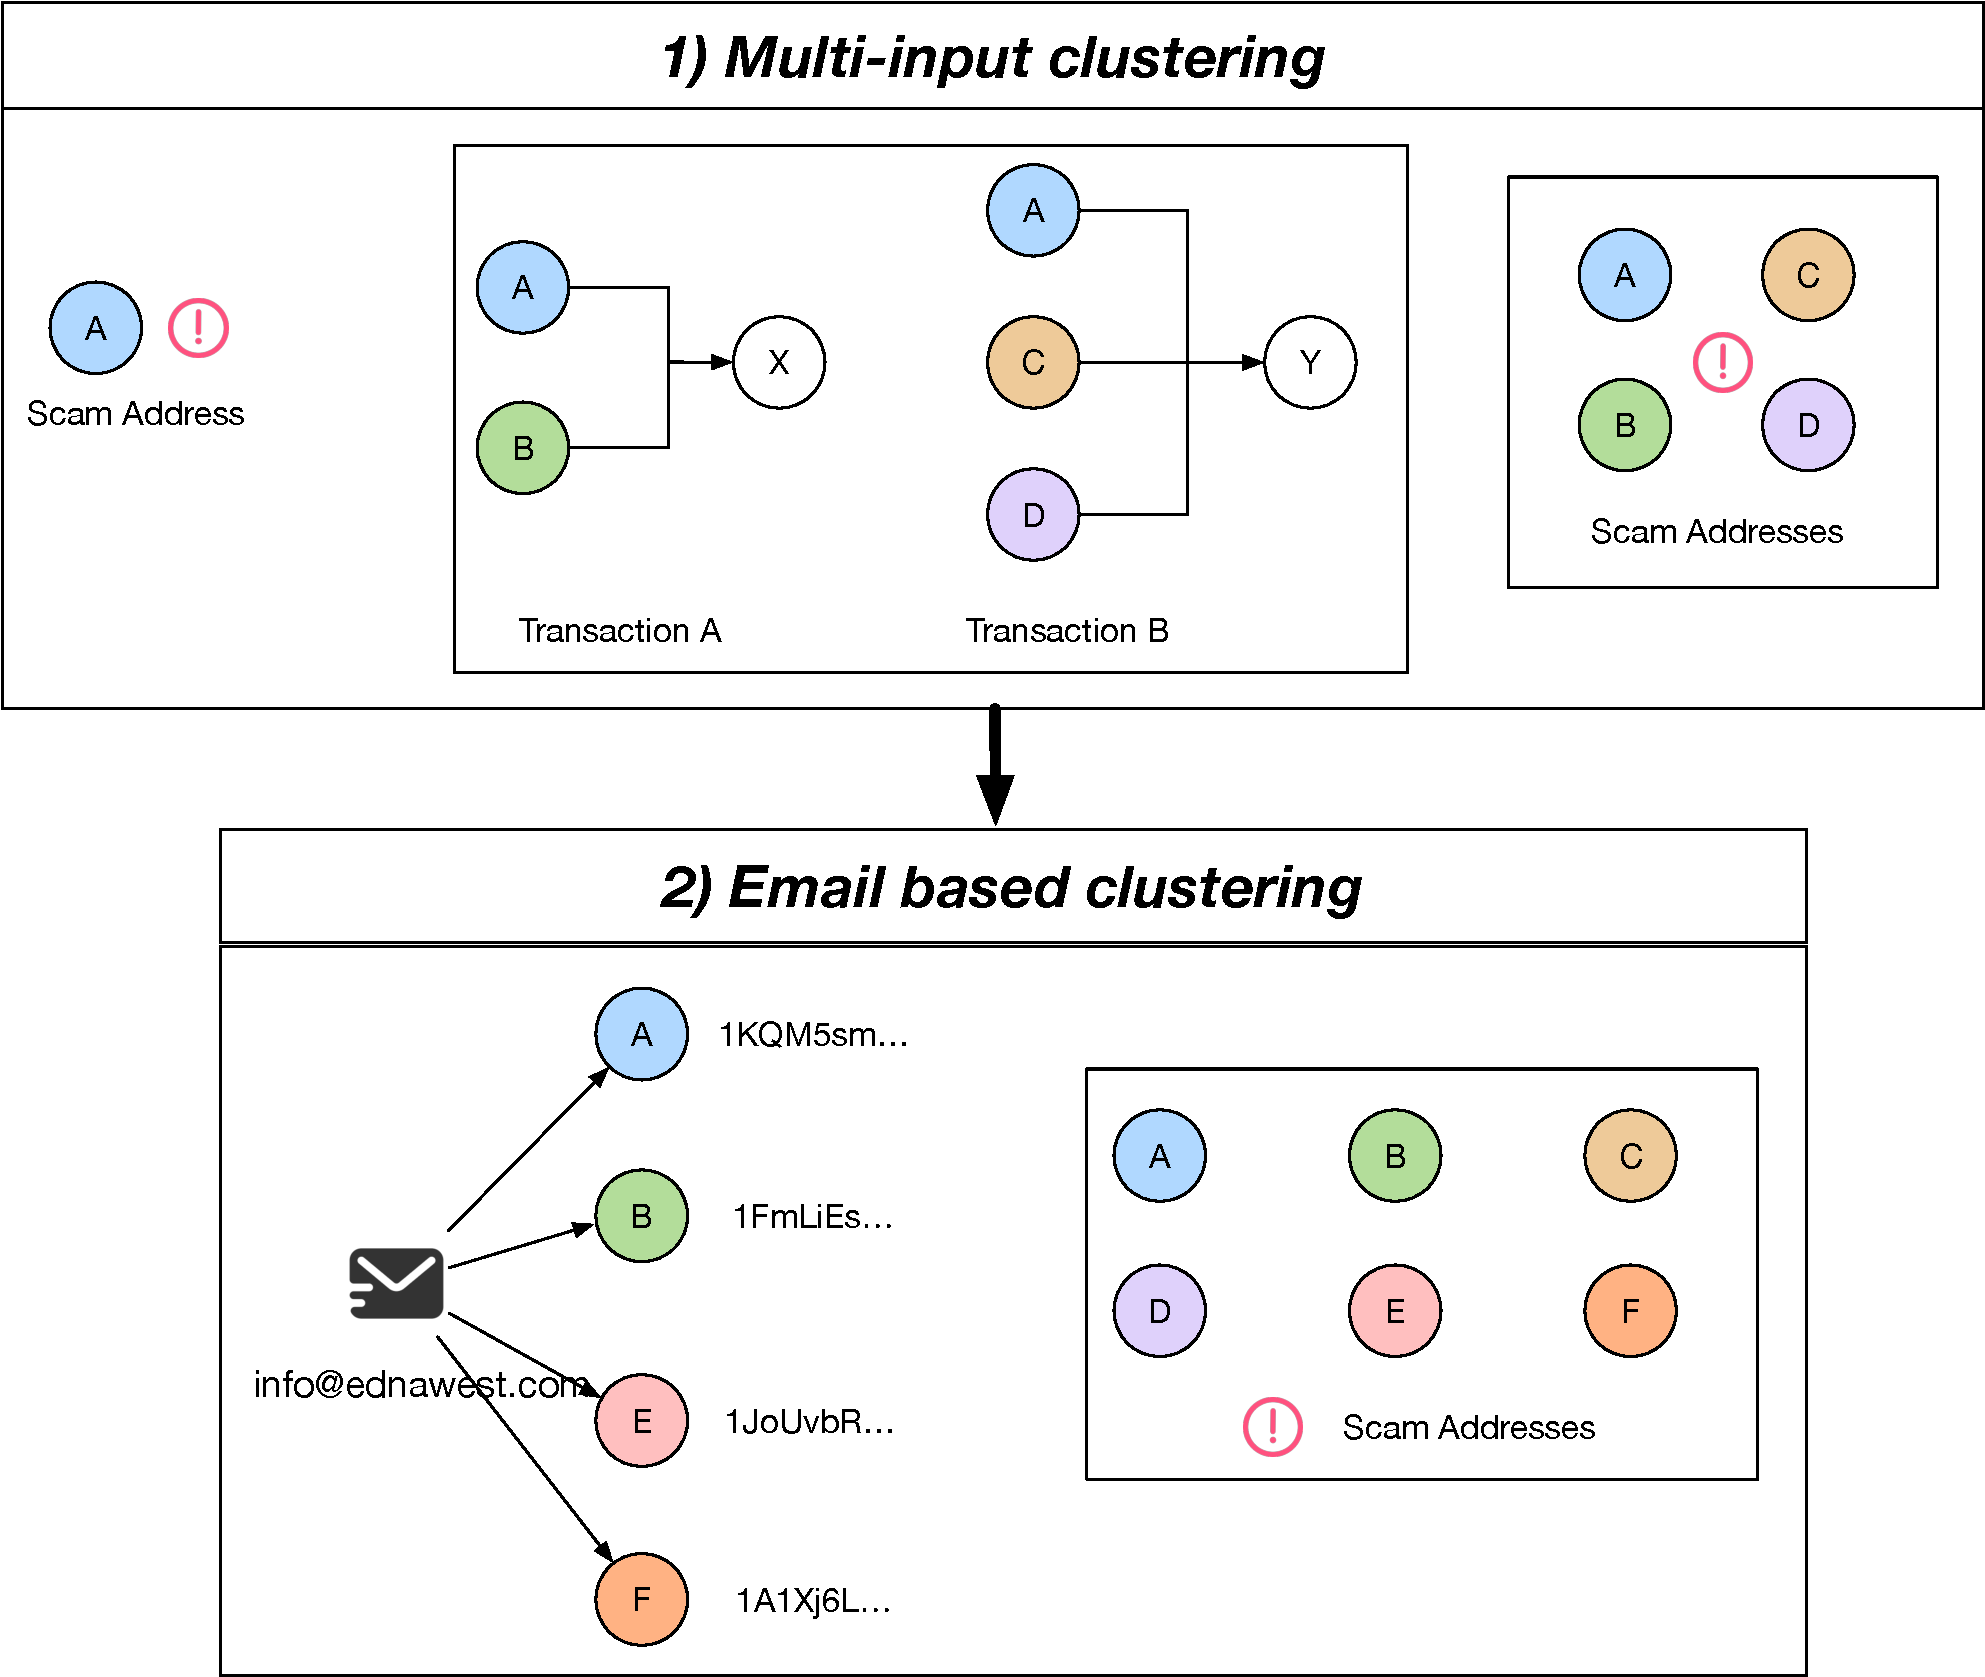
\includegraphics[width=\columnwidth]{images/clustering.pdf}}
\caption{The pipeline in clustering}
\label{fig:clustering-pipeline}
\end{figure}

\textbf{Transaction based multi-input clustering}
% explain multi-input clustering
We first use transaction based multi-input clustering to perform clustering on the dataset. The premise of multi-input clustering is that shared spending should infer shared control entity.


Research shows that compared to other clustering methods, multi-input clustering method is one with higher accuracy\cite{androulaki2013evaluating,harrigan2016unreasonable}.  By implementing multi-input clustering, we found out that 5,440(81.9\%)  addresses can be clustered together with other addresses. While there are still 1,203 addresses that can not be clustered using this method. These addresses only show up in the output addresses list in transactions, they never transfer their balance out to other addresses. We firstly implemented multi-input clustering for each labelled scam address, then we merge the clusters. In the end, we found 2,649 clusters. 15 clusters of them has more than 10,000 addresses.




\noindent\fbox{
\begin{minipage}{0.47\textwidth}{
\textbf{Answer to RQ3}: \textit{We clustered the addresses, and analysed the top 10 clusters, the result shows that these clusters got more than 1,620,599.08 bitcoins in total.  }
}\end{minipage}}

\textbf{Email-based clustering} The addresses that belong to the same email address can be regarded in the same illicit campaign. Our analysis shows that there are 7,134 (12.7\%) e-mail addresses which have more than 1 related bitcoin addresses. The result of email clustering is shown in table \ref{table:email-campaign}

\begin{table}[htbp]
\centering
 \caption{Email clustering result\label{table:email-campaign}}
 \begin{tabular}{cccc}
  \toprule
  Email Campaign & Sum1& Sum2 & Sum3 \\
  \midrule
 info@ednawest.com & 67 & 0 & 0\\
 lifeng@01aiche.com & 42 & 15 &6.8061\\
 maganuco@verbaereauto.com & 14 & 6 &1.39660959 \\
  pierre.leconte@verbaereauto.com& 17 & 7 & 1.3604\\
  anonymous@eldata.cz & 14 & 7 &5122.95105152 \\
  sqlbackup2019@pm.me & 20 & 10 & 1.17247444 \\
  rtrevieuly@outlook.com & 13 & 1 & 0.2850\\
   hxjtildiers@outlook.com&21 &0 &0 \\
  
  \bottomrule
 \end{tabular}
\end{table}




We than applied the result of email clustering to multi-input clustering, the final clustering result is given in table \ref{table:email-campaign}.In this table, Sum1 refers to the total amount of address in the campaign, Sum2 refers to the number of addresses that has ever received money. Sum3 refers to the amount of money the campaign received.

\begin{table}[htbp]
\centering
 \caption{Combined clustering result\label{table:email-campaign}}
 \begin{tabular}{cccc}
  \toprule
  Address Campaign & Sum1& Sum2 & Sum3 \\
  \midrule
 \#1 & 136,309 &129,497  &  487698.71 \\
 \#2 & 52,996 & 52,993 & 590764.78 \\
 \#3 & 40,186 & 40,186 &  41522.74\\
  \#4 & 39,084 & 39,084 & 54122.60 \\
  \#5 & 34,122 & 34,122 & 76208.43\\
  \#6 & 31,335 & 31,335 & 180457.08 \\
  \#7 & 26,856 & 26,856 & 24700.67 \\
   \#8 & 26,525 & 26,525 & 48608.16 \\
  \#9 &25,421 & 25,421 & 112552.48 \\
  \#10 & 20,576& 20,576 & 3963.43 \\
  \bottomrule
 \end{tabular}
\end{table}

\noindent\fbox{
\begin{minipage}{0.47\textwidth}{
\textbf{Answer to RQ5}: \textit{We cluster the scam address campaigns by two methods. One by multi-input clustering, we found out that the biggest cluster has more than 100,000 addresses in it. The total amount of bitcoin received by this cluster can reach xxx BTC. Another cluster method is by email, we found out that there are 12.7\% email addresses that have more than 1 related BTC address.}
}\end{minipage}}
